\subfigure[]{
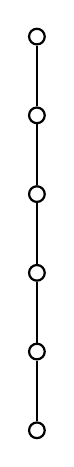
\begin{tikzpicture}
[nodedecorate/.style={shape=circle,inner sep=2pt,draw,thick},%
  linedecorate/.style={-,thick}]
%% nodes or vertices
\foreach \nodename/\x/\y in {1/0/0, 2/0/1, 3/0/2, 4/0/3, 5/0/4, 6/0/5} {
  \node (\nodename) at (\x,\y) [nodedecorate] {};
}
%% edges or lines
\path
\foreach \startnode/\endnode in {1/2, 2/3, 3/4, 4/5, 5/6} {
  (\startnode) edge[linedecorate] node {} (\endnode)
};
\end{tikzpicture}
}
\quad
%%
%%
\subfigure[]{
\begin{tikzpicture}
[nodedecorate/.style={shape=circle,inner sep=2pt,draw,thick},%
  linedecorate/.style={-,thick},%
  scale=1.5]
%% nodes or vertices
\foreach \nodename/\x/\y in {
  1/-0.8660/-0.5, 2/0.8660/-0.5, 3/0/1, 4/0/0, 5/0/2, 6/0/3} {
  \node (\nodename) at (\x,\y) [nodedecorate] {};
}
%% edges or lines
\path
\foreach \startnode/\endnode in {1/4, 2/4, 3/4, 3/5, 5/6} {
  (\startnode) edge[linedecorate] node {} (\endnode)
};
\end{tikzpicture}
}
\quad
%%
%%
\subfigure[]{
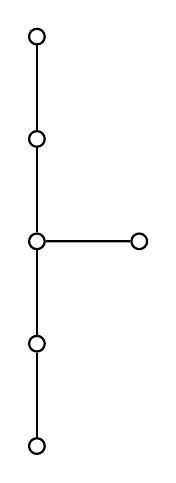
\begin{tikzpicture}
[nodedecorate/.style={shape=circle,inner sep=2pt,draw,thick},%
  linedecorate/.style={-,thick},%
  scale=1.3]
%% nodes or vertices
\foreach \nodename/\x/\y in {1/0/0, 2/0/1, 3/0/2, 4/0/3, 5/0/4, 6/1/2} {
  \node (\nodename) at (\x,\y) [nodedecorate] {};
}
%% edges or lines
\path
\foreach \startnode/\endnode in {1/2, 2/3, 3/4, 4/5, 3/6} {
  (\startnode) edge[linedecorate] node {} (\endnode)
};
\end{tikzpicture}
}
\quad
%%
%%
\subfigure[]{
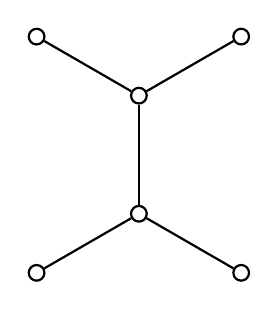
\begin{tikzpicture}
[nodedecorate/.style={shape=circle,inner sep=2pt,draw,thick},%
  linedecorate/.style={-,thick},%
  scale=1.5]
%% nodes or vertices
\foreach \nodename/\x/\y in {
  1/-0.8660/-0.5, 2/0.8660/-0.5, 3/0/1, 4/0/0, 5/-0.8660/1.5,
  6/0.8660/1.5}
{
  \node (\nodename) at (\x,\y) [nodedecorate] {};
}
%% edges or lines
\path
\foreach \startnode/\endnode in {1/4, 2/4, 3/4, 3/5, 3/6} {
  (\startnode) edge[linedecorate] node {} (\endnode)
};
\end{tikzpicture}
}
\quad
%%
%%
\subfigure[]{
\begin{tikzpicture}
[nodedecorate/.style={shape=circle,inner sep=2pt,draw,thick},%
  linedecorate/.style={-,thick},
  scale=1.3]
%% nodes or vertices
\foreach \nodename/\x/\y in {1/0/0, 2/0/1, 3/0/2, 4/0/3, 5/1/1, 6/-1/1} {
  \node (\nodename) at (\x,\y) [nodedecorate] {};
}
%% edges or lines
\path
\foreach \startnode/\endnode in {1/2, 2/3, 3/4, 2/5, 2/6} {
  (\startnode) edge[linedecorate] node {} (\endnode)
};
\end{tikzpicture}
}
\quad
%%
%%
\subfigure[]{
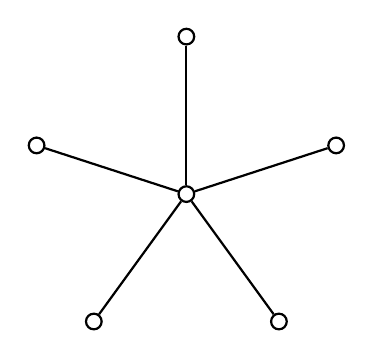
\begin{tikzpicture}
[nodedecorate/.style={shape=circle,inner sep=2pt,draw,thick},%
  linedecorate/.style={-,thick},%
  scale=2]
%% nodes or vertices
\foreach \nodename/\x/\y in {1/0.9510/0.3090, 2/0/1, 3/-0.9510/0.3090,
  4/-0.5877/-0.8090, 5/0.5877/-0.8090, 6/0/0}
{
  \node (\nodename) at (\x,\y) [nodedecorate] {};
}
%% edges or lines
\path
\foreach \startnode/\endnode in {1/6, 2/6, 3/6, 4/6, 5/6} {
  (\startnode) edge[linedecorate] node {} (\endnode)
};
\end{tikzpicture}
}
